% -*- root: ../SI2.tex -*-
\begin{problem}[1]
Se dispone de un equipo con un MTTF de 500 horas, que se encuentra bajo un contrato de mantenimiento que garantiza su reparación en un tiempo medio de 10 horas.
  \ppart El proveedor nos ofrece sustituirlo por un equipo de mayor calidad, con un MTTF de 1000 horas. Calcular la mejora de disponibilidad que supone este cambio.
  \ppart Tras un tiempo trabajando con el nuevo equipo, el proveedor nos ofrece de nuevo un nuevo equipo de mucha mayor calidad, con un MTTF de 2000 horas. Calcular la mejora de disponibilidad que supondría el nuevo cambio respecto al segundo equipo.

%%%%%%%%%%%%%%%%%%%%%%%%%%%%%%%%%%%%%%%%%%%%%%%%%%%%%%%%%%%%%%%%%%%%%
\solution
% \textcolor{red}{Hecho por Edu. Se ruegan correcciones.}
% Guille: A mí me parece bien.

\spart
  Calculemos la disponibilidad de cada equipo:
  \[ A_1 = \frac{500}{500+10} = \frac{50}{51} \approx 0.98039 \]
  \[ A_2 = \frac{1000}{1000+10} = \frac{100}{101} \approx 0.990099 \]
  Luego la mejora es inferior al $1\%$.

\spart
  \[ A_3 = \frac{2000}{2000+10} = \frac{200}{201} \approx 0.995 \]
  Lo que supone una mejora inferior al $0.5\%$ respecto al segundo y un $1.5\%$ respecto al original.

\end{problem}

%%%%%%%%%%%%%%%%%%%%%%%%%%%%%%%%%%%%%%%%%%%%%%%%%%%%%%%%%%%%%%%%%%%%%
\begin{problem}[2]
Se desea prestar un servicio con una indisponibilidad menor de 10 horas por año.
  \ppart Calcular la disponibilidad deseada del sistema.
  \ppart Se dispone de un servicio de mantenimiento que es capaz de sustituir un equipo averiado en 24 h. Calcular el MTTF que debe tener el equipo para poder satisfacer el requerimiento de disponibilidad establecido.

  \ppart Si sólo se dispone de equipos con un MTTF de 2000 horas, calcular el número de equipos que se deberían colocar en paralelo para garantizar el requisito.

%%%%%%%%%%%%%%%%%%%%%%%%%%%%%%%%%%%%%%%%%%%%%%%%%%%%%%%%%%%%%%%%%%%%%
\solution
% \textcolor{red}{Hecho por Edu. Se ruegan correcciones.}
% Guille: A mí me parece bien.

\spart
  Calculemos la disponibilidad:
  \[ A > \frac{365\cdot24-10}{365\cdot24} \implies A > 0.99886 \]

\spart
	Con un MTTR = 24h, podemos despejar el MTTF necesario utilizando la A calculada en el apartado anterior:
	\begin{gather*}
	0.99886 = \frac{\textit{MTTF}}{\textit{MTTF}+24} \iff \textit{MTTF} · (1-0.99886)=24\cdot0.99886\\
	\textit{MTTF} = \frac{24\cdot0.99886}{1-0.99886} \approx 21028.6316 \text{ horas (} \approx\text{2.5 años)}
	\end{gather*}

\spart
	Calculemos la disponibilidad de un único equipo
	\[ A_e = \frac{2000}{2000+24} \approx 0.98814 \]
	Ahora calculemos el número de equipos utilizando la fórmula para componentes redundantes:

	\begin{align*}
	0.99886 &\geq 1 - (1 - 0.98814)^n \\
	(1 - 0.98814)^n &\geq 1 - 0.99886\\
	n\cdot \log(1 - 0.98814) &\geq  \log(1 - 0.99886) \\
	n &\geq 1.52
	\end{align*}

	Como buscamos el mínimo $n$ tal que cumpla esa desigualdad y $n \in \nat \implies n = 2$.

\end{problem}

%%%%%%%%%%%%%%%%%%%%%%%%%%%%%%%%%%%%%%%%%%%%%%%%%%%%%%%%%%%%%%%%%%%%%
\begin{problem}[3]
El servidor de envío de mensajes ("busca") descrito en el problema número 7 del Tema 2 (\ref{tema2:prob7}) se compone de dos dispositivos: uno de recepción de mensajes y otro de difusión de los mismos.
\begin{itemize}
\item El MTTF del dispositivo de recepción de mensajes es de 1000 horas.
\item El MTTF del dispositivo de difusión es de 1500 horas.
\end{itemize}
Ambos los atiende el mismo servicio técnico, que en ambos casos nos asegura un MTTR de 5 horas.

Se pide calcular la disponibilidad total del sistema.

%%%%%%%%%%%%%%%%%%%%%%%%%%%%%%%%%%%%%%%%%%%%%%%%%%%%%%%%%%%%%%%%%%%%%
\solution
% \textcolor{red}{Hecho por Edu. Se ruegan correcciones.}
% Guille: A mí me parece bien.

Como son 2 elementos en serie, la disponibilidad total es el producto de las disponibilidades. Como $ A_{\text{receptor}} = \frac{1000}{1000+5}$ y $A_{\text{difusor}} = \frac{1500}{1500+5}$, tenemos que \[ A_{\text{total}} = \frac{1500\cdot1000}{1505\cdot1005} \approx 0.9917 \]

\end{problem}

%%%%%%%%%%%%%%%%%%%%%%%%%%%%%%%%%%%%%%%%%%%%%%%%%%%%%%%%%%%%%%%%%%%%%
\begin{problem}[4]
Los datos de disponibilidad de cada uno de los componentes de la red de la entidad financiera descrita en el problema número 8 del Tema 2 (\ref{tema2:prob8}) son los siguientes:
\begin{itemize}
	\item MTTF del multiplexor: 2000 h.
	\item MTTF del servidor: 2000 h.
	\item MTTF de cada terminal remoto: 1000 h.
	\item MTTF de la línea de comunicaciones del terminal remoto: 500 horas.
	\item MTTR de todos los elementos: 5 horas.
\end{itemize}

Suponiendo la existencia de dos únicos terminales remotos, realizar el diagrama de bloques de disponibilidad y calcular la disponibilidad global del sistema.

%%%%%%%%%%%%%%%%%%%%%%%%%%%%%%%%%%%%%%%%%%%%%%%%%%%%%%%%%%%%%%%%%%%%%
\solution
% \textcolor{red}{Hecho por Edu. Se ruegan correcciones.}
% Guille: A mí me parece bien.

Aquí hay que interpretar un poco el problema\footnote{se aceptan críticas.}, lo que yo entiendo es un esquema como el de la figura \ref{tema3:prob4:esquema}.
\begin{figure}[hbtp]
	\centering
	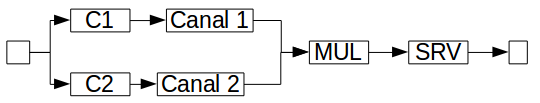
\includegraphics[keepaspectratio=true,width=0.8\linewidth]{img/tema3_ej4.png}
	\caption{Esquema.}
	\label{tema3:prob4:esquema}
\end{figure}

Siguiendo este esquema, hay que calcular la disponibilidad de cada cliente en serie con su canal, luego calcular la disponibilidad en paralelo de los clientes, y luego calcular la disponibilidad de los clientes, el multiplexor y el servidor en serie. Vamos a ello:
\begin{itemize}
\item \textbf{De un par cliente-canal}:
\[ A_1 = \frac{1000}{1000+5} \cdot \frac{500}{500+5} = \frac{20000}{20301} \approx 0.9852 \]
\item \textbf{De los clientes}:
\[ A_{\text{Clientes}} = 1 - (1 - 0.9852)^2 \approx 0.9998 \]
\item \textbf{Del multiplexor y el servidor}:\footnote{que tienen el mismo MTTF.}
\[ A_{\text{MUL}} = \frac{2000}{2000+5} = \frac{2000}{2005} \approx 0.9975 \]
\item \textbf{De la red}:\\
Juntándolo todo obtenemos lo siguiente:
\[ A = 0.9998 \cdot 0.9975 \cdot 0.9975 \approx 0.9948 \]
\end{itemize}

\end{problem}

%%%%%%%%%%%%%%%%%%%%%%%%%%%%%%%%%%%%%%%%%%%%%%%%%%%%%%%%%%%%%%%%%%%%%
\begin{problem}[5]
Un servidor de fecha y hora de una red se compone de dos elementos, que deben estar operativos para atender el servicio: Un ordenador, que satisface las peticiones, y un receptor
de señales horarias externo, que permite obtener la hora exacta. Si ambos equipos tienen un MTTF de 1500 horas, calcular el MTTR mínimo que debemos considerar, supuesto igual en ambos, si se desea una disponibilidad total del servicio mayor del $99\%$.

%%%%%%%%%%%%%%%%%%%%%%%%%%%%%%%%%%%%%%%%%%%%%%%%%%%%%%%%%%%%%%%%%%%%%
\solution
% \textcolor{red}{Hecho por Edu. Se ruegan correcciones.}
% Guille: A mí me parece bien.

Como son componentes en serie, la disponibilidad es el producto:
\begin{align*}
A = \frac{1500}{1500+\text{MTTR}} \cdot \frac{1500}{1500+\text{MTTR}} &> 0.99\\[0.2em]
1500^2 &> 0.99 \cdot (1500+\text{MTTR})^2 \\[0.2em]
\frac{1500^2}{0.99} = \frac{1500^2 \cdot 10^2}{99} &> 1500^2 + 3000 \cdot \text{MTTR} + \text{MTTR}^2 \\
0 &> 1500^2\left(1 -\frac{100}{99}\right) + 3000 \cdot \text{MTTR} + \text{MTTR}^2
\end{align*}

Primero resolvemos la ecuación de segundo grado:
\[ \text{MTTR} = \frac{-3000 \pm \sqrt{3000^2 - 4 \cdot 1 \cdot 1500^2(1 -\frac{100}{99})}}{2} = \frac{-3000 \pm 3015.1134}{2} \]

Como el resultado de $\text{MTTR}=-3007.5567$ horas es absurdo, $\text{MTTR}=7.5567$ horas es el único resultado que tiene sentido.\\

Como lo que queremos resolver es la inecuación, el resultado es $\text{MTTR} < 7.5567$.
\end{problem}

%%%%%%%%%%%%%%%%%%%%%%%%%%%%%%%%%%%%%%%%%%%%%%%%%%%%%%%%%%%%%%%%%%%%%
\begin{problem}[6]
Un servicio que debe tener una disponibilidad mínima de 0.99 se debe proporcionar con un sistema cuyo tiempo medio hasta el fallo es de 2000 horas.
\ppart
Calcular el tiempo medio para reparar el equipo que es necesario para satisfacer la disponibilidad solicitada.
\ppart
Al comenzar con la explotación del servicio se descubre que el programa que lo implementa tiene fallos que hacen que en ocasiones se bloquee, dejando de atender peticiones. Para resolverlo es necesario detener el proceso y volverlo a arrancar. Se ha estimado que en media se produce un fallo cada dos días. El fallo se tarda en descubrir un promedio de 5 min. y la reiniciación del proceso requiere, también en promedio, 7 min. Calcular la disponibilidad del sistema considerando este efecto.
\ppart
Suponiendo imposible modificar el programa o cambiar el equipo, proponer una alternativa que permita, en las nuevas circunstancias, satisfacer el requerimiento inicial de disponibilidad.

%%%%%%%%%%%%%%%%%%%%%%%%%%%%%%%%%%%%%%%%%%%%%%%%%%%%%%%%%%%%%%%%%%%%%
\solution
% \textcolor{red}{Hecho por Edu. Se ruegan correcciones.}
% Guille: A mí me parece bien.

\spart
\[ A = \frac{2000}{2000+\text{MTTR}} > 0.99 \iff \frac{2000}{0.99} - 2000 > \text{MTTR} \iff 20.\gor{20} > \text{MTTR} \]
Luego tomando el MTTR más grande posible, $MTTR = 20.202$ horas es suficiente.\footnote{Añadidle todos los 020's que queráis detrás.}

\spart
Con estos datos, decimos que $MTTF_{\text{programa}} = 48$ horas (2880 min), $MTTR_{\text{programa}} = 5+7 = 12$ min
\[ A_{\text{programa}} = \frac{2880}{2880+12} = \frac{240}{241} \approx 0.99585\]
Luego:
\[ A_{\text{total}} = 0.99 \cdot 0.99585 \approx 0.98589 \]
Y descubrimos, con estupor, que no cumplimos el contrato.

\spart
``Debido a que tenemos el deber de cumplirlo, nos embarcamos en la búsqueda de una solución.
Primero, consideramos poner elementos en paralelo, pero como no podemos cambiar el programa para solucionar sus fallos ni añadirle funcionalidad para que se pueda repartir la carga entre varios, no podemos llevar a cabo esta solución. En segundo lugar, se nos ocurre aumentar el tiempo medio hasta el fallo, pero el \textit{sysadmin} nos amenaza con cortarnos las gónadas si le tocamos su sistema, y la empresa que proporciona el programa tampoco es capaz de solucionarnos el problema resolviendo los \textit{bugs}. No desesperando en nuestro empeño, perseveramos, y observamos que, desembolsando algunos euros más, podemos contratar un becario para mejorar la disponibilidad reduciendo el MTTR. ¡Albricias! -pensamos, pero, ¿cuánto debemos reducirlo?''\\

Tras esta bonita historia, vamos a resolver el problema:\\
Observamos que hay dos MTTRs que podemos mejorar, pero el del programa ya es bastante bajo en comparación con el del sistema (12 min frente a 20.20 horas)\footnote{obsérvese que la disponibilidad no tiene unidades.}, luego es evidente que mejorando el del sistema podemos cumplir con el contrato:
\[ 0.99 = 0.99585 \cdot \frac{2000}{2000+\text{MTTR}} \iff \text{MTTR} = \frac{0.99585 \cdot 2000}{0.99} - 2000 \approx 11.\gor{81} \text{ horas}\]
Y, tomando un MTTR $=11.818$ horas para el sistema, comprobamos que la nueva disponibilidad es:
\[ A = \frac{2000}{2000+11.818} \cdot 0.99585 \approx 0.99... > 0.99 \]
Y nos vamos felices, sabiendo que hemos hecho un \textit{buen trabajo}.
\end{problem}

%%%%%%%%%%%%%%%%%%%%%%%%%%%%%%%%%%%%%%%%%%%%%%%%%%%%%%%%%%%%%%%%%%%%%
\begin{problem}[7]
Una petición que se procesa en un servidor web tiene que pasar por cuatro clases de elementos distintos para su resolución completa. Estos elementos son:
\begin{itemize}
	\item Un distribuidor de carga, que reparte las peticiones a los servidores web.
	\item Un servidor web, que entrega al cliente páginas estáticas e imágenes. Existen en el sistema tres servidores web, de igual funcionalidad, pudiendo cualquiera de ellos atender las peticiones.
	\item Un servidor de aplicaciones, que ejecuta programas bajo petición de los servidores web. El sistema posee dos de estos servidores, de igual funcionalidad. Los servidores web pueden enviar indistintamente sus peticiones a cualquiera de ellos.
	\item Un servidor de base de datos, al cual acceden los programas que se ejecutan en los servidores de aplicaciones para recuperar los datos que necesitan para realizar las peticiones.
\end{itemize}

Es necesario, por tanto, que esté disponible al menos un elemento de cada una de las clases citadas anteriormente para que el sistema completo funcione.
\ppart
Dibujar el diagrama de disponibilidad del sistema total definido.

\ppart
Suponiendo que todos los ordenadores que implementan los servidores tienen la misma disponibilidad, A, y que cada servidor se implementa en un ordenador distinto, calcular la expresión de la disponibilidad total del sistema, AT en función de A.

\ppart
Calcular el valor numérico de AT cuando el tiempo medio entre fallos es de 2000 horas y el tiempo medio entre reparaciones, 100 horas.

%%%%%%%%%%%%%%%%%%%%%%%%%%%%%%%%%%%%%%%%%%%%%%%%%%%%%%%%%%%%%%%%%%%%%
\solution
\textcolor{red}{Hecho por Edu. Se ruegan correcciones.}\\

\spart
El esquema es el mostrado en la figura \ref{tema3:prob7:esquema}.
\begin{figure}[hbtp]
	\centering
	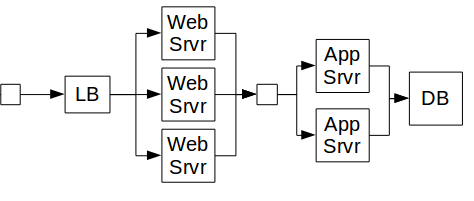
\includegraphics[keepaspectratio=true,width=\linewidth]{img/tema3_ej7.png}
	\caption{Esquema de cadena de procesamiento.}
	\label{tema3:prob7:esquema}
\end{figure}
$ $\\
\spart
Aplicando la misma idea que en la transparencia 17:
\[ AT = A \cdot (1 - (1 - A)^3) \cdot (1 - (1 - A)^2) \cdot A \eqreason{sage} -A^7 + 5*A^6 - 9*A^5 + 6*A^4 \]

\spart
Sabiendo que $A = \frac{2000}{2000+100} = \frac{200}{201}$:
\[ AT \eqreason{sage} \frac{13122889600000000}{13254776280841401} \approx 0.99 \]
\end{problem}

%%%%%%%%%%%%%%%%%%%%%%%%%%%%%%%%%%%%%%%%%%%%%%%%%%%%%%%%%%%%%%%%%%%%%
\begin{problem}[8]
Cada uno de los elementos que componen el servidor de transacciones descrito en el problema número 15 del Tema 2 (\ref{tema2:prob15}) se ejecuta en un ordenador independiente que tiene un MTTF de 4000 horas. Calcular el MTTR necesario para garantizar una disponibilidad del sistema total del 99.9\%.

%%%%%%%%%%%%%%%%%%%%%%%%%%%%%%%%%%%%%%%%%%%%%%%%%%%%%%%%%%%%%%%%%%%%%
\solution
\textcolor{red}{Hecho por Edu. Se ruegan correcciones.}\\

Tenemos:
\[ A_{\text{proceso}} = A_{\text{DB}} = \frac{4000}{4000+\text{MTTR}}\]

Debido a que hay un bucle, hay que ver cuántas vueltas se dan. El número de vueltas sigue una geométrica\footnote{del tipo: ``número de fallos hasta primer acierto''. Ver \url{http://en.wikipedia.org/wiki/Geometric_distribution}.}, con esperanza $\frac{1-q}{q}$, llamando a eso n, tenemos que:
\[ A_T = A_{\text{proceso}}^{n+1} \cdot A_{\text{DB}}^{n} \]

Esto es: si se dan 0 vueltas, la disponibilidad del sistema es la del primer componente; si se da una, es como si la cadena fuera el primer componente, seguido de la DB, seguido del proceso; y así sucesivamente.

Luego
\begin{gather*}
0.999 = (\frac{4000}{4000+\text{MTTR}})^{n+1} \cdot (\frac{4000}{4000+\text{MTTR}})^{n} \eqreason{sage} \left(\frac{4000}{\text{MTTR} + 4000}\right)^{2n + 1}\\
(\text{MTTR} + 4000)^{2n + 1} = \frac{4000^{2n + 1}}{0.999} \\
\text{MTTR} + 4000 = \sqrt[2n+1]{\frac{4000^{2n + 1}}{0.999}}\\
\text{MTTR} = \sqrt[2n+1]{\frac{4000^{2n + 1}}{0.999}} - 4000\\
\end{gather*}

Luego en función de n (que dependen del q del problema \ref{tema2:prob15}), podemos calcular el MTTR.\\

\newpage
\textcolor{blue}{Hecho por Herea.}\\
MTTF$_{\text{proceso}} = MTTF_{\text{BD}} = 4000$ horas.\\
Disponibilidad exigida 99.9\%. ¿MTTR?
\begin{gather*}
0.999 = \left(\frac{4000}{4000+\text{MTTR}}\right)^2 \\
(4000+\text{MTTR})^2 = \frac{4000^2}{0.999} \\
4000^2 + 8000 \text{MTTR} + \text{MTTR}^2 - \frac{4000^2}{0.999} = 0\\
\text{MTTR} = \frac{-8000 \pm \sqrt{8000^2 - 4 \cdot (-16016.016)}}{2} = \\
= \frac{-8000 \pm 8004.003}{2} = \frac{4.003}{2} = 2.0015 \text{ horas}
\end{gather*}
\end{problem}

%%%%%%%%%%%%%%%%%%%%%%%%%%%%%%%%%%%%%%%%%%%%%%%%%%%%%%%%%%%%%%%%%%%%%
\begin{problem}[9]
Comparar desde el punto de vista de disponibilidad las dos soluciones propuestas en el problema número 18 del Tema 2 (\ref{tema2:prob18}) para resolver un cuello de botella en acceso a disco. Suponer que todos los discos empleados tienen los mismos MTTF y MTTR, y justifique qué alternativa es más fiable calculando y comparando las disponibilidades en ambos casos.

%%%%%%%%%%%%%%%%%%%%%%%%%%%%%%%%%%%%%%%%%%%%%%%%%%%%%%%%%%%%%%%%%%%%%
\solution


\end{problem}

%%%%%%%%%%%%%%%%%%%%%%%%%%%%%%%%%%%%%%%%%%%%%%%%%%%%%%%%%%%%%%%%%%%%%
\begin{problem}[10]
Los servidores de directorios DSA1 y DSA2 descritos en el problema número 20 del Tema 2 (\ref{tema2:prob20}) se encuentran conectados por una línea de comunicaciones que tiene una disponibilidad de 0.99. La disponibilidad de DSA2 es de 0.98. Si el MTTF de DSA1 es de 2000 horas, ¿cuál será el MTTR que deberemos garantizar para él, para conseguir que la disponibilidad del sistema total se igual a 0.95? ¿Cuál sería, en este caso, la disponibilidad de DSA considerado aislado del resto del sistema?

%%%%%%%%%%%%%%%%%%%%%%%%%%%%%%%%%%%%%%%%%%%%%%%%%%%%%%%%%%%%%%%%%%%%%
\solution


\end{problem}

%%%%%%%%%%%%%%%%%%%%%%%%%%%%%%%%%%%%%%%%%%%%%%%%%%%%%%%%%%%%%%%%%%%%%
\begin{problem}[11]
Se desea definir la arquitectura de un servidor de aplicaciones siguiendo el modelo estándar visto en la asignatura, compuesto por cuatro elementos distintos en la cadena de procesamiento:
\begin{itemize}
	\item Capa de distribución: Balanceador de carga del tráfico de usuarios.
La alta disponibilidad de estos elementos se garantizará mediante el
protocolo VRRP.
	\item Capa de presentación: Servidores web. La capa anterior garantiza una alta disponibilidad activo-activo en esta capa.
	\item Capa de aplicación: Servidores de aplicaciones. El web plug-in
insertado en los servidores web garantiza la alta disponibilidad
activo-activo en esta capa.
	\item Capa de datos: Servidores de bases de datos. Se elige que la
alta disponibilidad de esta capa la proporcione un cluster
activo-pasivo.

\end{itemize}

Los ordenadores con los que se trabaja tienen un MTTF de 4000 horas, y su MTTR es de 48 horas.
\ppart Calcular la disponibilidad de la capa de presentación si se colocan en ella dos servidores web.
\ppart Adicionalmente a los posibles problemas de hardware reflejados en el MTTF genérico de los servidores empleados, se han detectado fallos en el software de los servidores de aplicaciones, que hacen que en promedio exista un fallo por semana que hace necesario rearrancar el servidor. El tiempo de rearranque del servidor es de 30 min. Calcular la
disponibilidad de la capa de aplicación si se colocan en ella dos servidores de aplicaciones.
\ppart En el caso de la base de datos, la recuperación tras un fallo no se realiza a través de las reparaciones habituales, sino que se dispone de un cluster activo-pasivo. El tiempo de conmutación al servidor pasivo se compone de los siguientes tiempos:
\begin{itemize}
	\item Tiempo de detección del fallo en el servidor principal: 30s.
	\item Tiempo de arranque del servidor pasivo: 30 min.
	\item Tiempo de recuperación de la base de datos tras un cierre anormal, en el caso peor: 2 horas.
\end{itemize}

Calcular la disponibilidad de la capa de datos en dicho caso peor.
\ppart En la capa de distribución se conocen los siguientes datos:
\begin{itemize}
	\item Advertisement interval (tiempo entre la transmisión de paquetes hello por el balanceador activo): 1s.
	\item Master down interval (tiempo tras el cual si no se reciben paquetes hello se considera el master caído): 3s.
	\item Skew adicional para producir la conmutación tras la expiración del master down interval: 0.
\end{itemize}

Calcular, en el caso peor, la disponibilidad del conjunto de dos balanceadores de carga trabajando en esta configuración.
\ppart Calcular la disponibilidad total de la instalación.

%%%%%%%%%%%%%%%%%%%%%%%%%%%%%%%%%%%%%%%%%%%%%%%%%%%%%%%%%%%%%%%%%%%%%
\solution


\end{problem}
